\documentclass[a4paper,12pt]{article}
\usepackage{amssymb}
\usepackage{amsmath}
\usepackage{amsthm} 
\usepackage{caption}
\usepackage{misccorr}
\usepackage[noadjust]{cite}
\usepackage{cmap} 
\usepackage[utf8]{inputenc}
\usepackage[T2A]{fontenc}
\usepackage[english, russian]{babel}
\usepackage{indentfirst}
\setlength{\parindent}{5ex}
\usepackage{graphics}
\usepackage{graphicx}
\usepackage{textcomp}
\usepackage{verbatim}
\usepackage{makeidx}
\usepackage{geometry}
\usepackage{float}
\usepackage{bm}
\usepackage{esint}
\usepackage{mathtools}
\usepackage{graphicx}
\usepackage{listings}
\usepackage{courier}
\usepackage{multirow}
\usepackage{graphicx}

\lstset{basicstyle=\fontsize{10}{10}\selectfont,breaklines=true}

\newcommand{\specchapter}[1]{\chapter*{#1}\addcontentsline{toc}{chapter}{#1}}
\newcommand{\specsection}[1]{\section*{#1}\addcontentsline{toc}{section}{#1}}
\newcommand{\specsubsection}[1]{\subsection*{#1}\addcontentsline{toc}{subsection}{#1}}
\newcommand{\RNumb}[1]{\uppercase\expandafter{\romannumeral #1\relax}}
\newcommand{\jj}{\righthyphenmin=20 \justifying}


% геометрия
\geometry{pdftex, left = 2cm, right = 2cm, top = 2.5cm, bottom = 2.5cm}

\setcounter{tocdepth}{4} % фикс переноса 
\righthyphenmin = 2
\tolerance = 2048

\begin{document}
\thispagestyle{empty}

\noindent \begin{minipage}{0.15\textwidth}
	
\includegraphics[width=\linewidth]{b_logo}
\end{minipage}
\noindent\begin{minipage}{0.9\textwidth}\centering
	\textbf{Министерство науки и высшего образования Российской Федерации}\\
	\textbf{Федеральное государственное бюджетное образовательное учреждение высшего образования}\\
	\textbf{«Московский государственный технический университет имени Н.Э.~Баумана}\\
	\textbf{(национальный исследовательский университет)»}\\
	\textbf{(МГТУ им. Н.Э.~Баумана)}
\end{minipage}

\noindent\rule{18cm}{3pt}
\newline\newline
\noindent ФАКУЛЬТЕТ $\underline{\text{«Информатика и системы управления»}}$ \newline\newline
\noindent КАФЕДРА $\underline{\text{«Программное обеспечение ЭВМ и информационные технологии»}}$\newline\newline\newline\newline\newline\newline\newline


\begin{center}
	\noindent\begin{minipage}{1.3\textwidth}\centering
	\Large\textbf{  Лабораторная работа № 6}\newline
	\textbf{по дисциплине "Вычислительные алгоритмы"}\newline\newline\newline
	\end{minipage}
\end{center}

\noindent\textbf{Тема} $\underline{\text{Построение   и  программная   реализация   алгоритмовчисленного дифференцирования.}}$\newline\newline
\noindent\textbf{Студент} $\underline{\text{Мицевич М. Д.}}$\newline\newline
\noindent\textbf{Группа} $\underline{\text{ИУ7-41Б}}$\newline\newline
\noindent\textbf{Оценка (баллы)} $\underline{\text{~~~~~~~~~~~~~~~~~~~~~~~~~~~}}$\newline\newline
\noindent\textbf{Преподаватель} $\underline{\text{Градов В.М.}}$\newline

\begin{center}
	\vfill
	Москва~---~\the\year
~г.
\end{center}
\clearpage

\section{Цель работы}

\noindent Получение навыков построения алгоритмавычисления производных от сеточных функций .

\section{Исходные данные}
Задана табличная (сеточная) функция. Имеется информация, что закономерность, представленная этой таблицей, может быть описана  формулой
\[y = \frac{a_0x}{a_1 + a_2x}\]
\begin{tabular}{|c|c|c|c|c|c|c|}
    \hline
    x & y & 1 & 2 & 3 & 4 & 5 \\
    \hline
    1 & 0.571 & & & & & \\
    \hline
    2 & 0.889 & & & & & \\
    \hline
    3 & 1.091 & & & & & \\
    \hline
    4 & 1.231 & & & & & \\
    \hline
    5 & 1.333 & & & & & \\
    \hline
    6 & 1.412 & & & & & \\
    \hline
\end{tabular}

Вычислить первые разностные производные от функции и занести их в столбцы (1)-(4) таблицы:
\newline1 - односторонняяразностная производная,
\newline2 -центральнаяразностная производная,
\newline3-2-я формула Рунге с использованием одностороннейпроизводной,
\newline4 -введены выравнивающие переменные.
\newlineВ столбец 5 занестивторую разностную производную.

\section{Код программы}
\noindent\textbf{Листинг main.py:}
\lstinputlisting[frame=single, language=Python]{main.py}

\section{Результаты}
\begin{figure}[H]
    \centering
    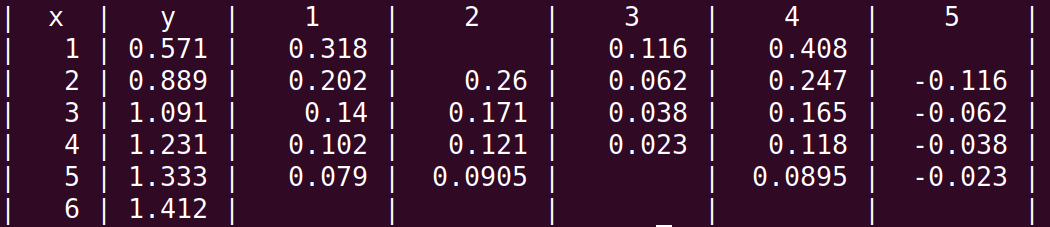
\includegraphics[scale=0.4]{./screens/table.png}
    \caption{Таблица результатов}
    \label{fig:my_label}
\end{figure}

\subsection{Правая разностная производная}
\underline{Формула:}
\[y'_n = \frac{y_{n+1} - y_n}{h} + O(h)\]

\underline{Точность:} первый порядок точности относительно шага h

\subsection{Центральная разностная производная}
\underline{Формула:}
\[y'_n = \frac{y_{n+1} - y_{n-1}}{2h} + O(h^2)\]

\underline{Точность:} второй порядок точности относительно шага h

\subsection{2-я формула Рунге с использованием односторонней производной}
\underline{Формула:}
\[\Omega = \Phi(h) + \frac{\Phi(h) - \Phi(mh)}{m^p-1} + O(h^{p+1})\]

\underline{Точность:} точность формулы Рунге повышается за счет расчет на 2 сетках с отличающимеся шагами. Точность формулы - p+1. В программе я использовал формулу Рунге для правой разностной производной, поэтому m = 2 - удвоенный шаг, p = 1.

\subsection{Введение выравнивающих переменных}
Требуется подобрать такие $\eta(y)$ и $\xi(x)$, чтобы функция $\eta(\xi)$ была линейной. Исходя из заданной формы фунцкии в условии задачи, зададим $\eta(y) = \frac{1}{y}$ и $\xi(x) = \frac{1}{x}$, тогда $\eta(\xi) = \frac{a_1}{a_0}\xi + \frac{a_0}{a_2}$, что и требовалось.

Тогда для возврата к исходным переменным используется формула:
\[y_x' = y_{\eta}'\eta_{\xi}'\xi_{x}' = \frac{\eta_{\xi}'\xi_x'}{\eta_y'}\]

Воспользуемся формулой правой разностной производной и получим:
\[y_n' = \frac{\frac{1}{y_{n+1}} - \frac{1}{y_n}}{\frac{1}{x_{n+1}} - \frac{1}{x_n}}\frac{y_n^2}{x_n^2}\]

\underline{Точность:} Формула абсолютно точная

\subsection{Вторая разностная производная}
\underline{Формула:}
\[y''_n = \frac{y_{n-1} - 2y_n + y_{n+1}}{h^2} + O(h^2)\]

\underline{Точность:} второй порядок точности относительно шага h

\section{Контрольные вопросы}
\subsection{Получить формулу порядка точности $О(h^2)$ для первой разностной производной $y'_N$ в крайнем правом узле $x_N$.}
Запишем ряды Тейлора в точках n-1 и n-2:

\begin{equation}
    y_{n-1} = y_{n} + \frac{h}{1!}y_n' + \frac{h^2}{2!}y_n'' + ...
\end{equation}

\begin{equation}
    y_{n-2} = y_{n} + \frac{2h}{1!}y_n' + \frac{(2h)^2}{2!}y_n'' + ...
\end{equation}

Вычтем из 4 первых второе:
\[4y_{n-1} - y_{n-2} = 3y_n + 2h y_n' + O(h^2)\]

Отсюда:
\[y_n' = \frac{4y_{n-1} - y_{n-2} - 3y_n}{2h} + O(h^2)\]

\subsection{Получить формулу порядка точности $O(h2)$ для второйразностной производной $y_0''$ в крайнем левом  узле $x_0$.}
Запишем ряды Тейлора в точках 1 и 2:

\begin{equation}
    y_{1} = y_{0} + \frac{h}{1!}y_0' + \frac{h^2}{2!}y_0'' + \frac{h^3}{3!}y_0''' ...
\end{equation}

\begin{equation}
    y_{2} = y_{0} + \frac{2h}{1!}y_0' + \frac{(2h)^2}{2!}y_0'' + \frac{(2h)^3}{3!}y_0''' ...
\end{equation}

Вычтем из 8 третьих четвертое:
\[8y_1 - y_2 = 7y_0 + 6h y_0' + 2h^2 y_0'' + O(h^2)\]

Отсюда:
\[y_0'' = \frac{8y_1 - y_2 - 7y_0 - 6h\frac{-3y_0 + 4y_1 - y_2}{2h}}{2h^2} + O(h^2)\]

\subsection{Используя 2-ую формулу Рунге, дать вывод выражения(9) из Лекции №7 для первой производной $y_0'$ в левом крайнем узле }

\begin{align*}
    \Omega &= \Phi(h) + \frac{\Phi(h) - \Phi(2h)}{2^1-1} + O(h^{1+1}) \\
    \Phi(h) &= \frac{y_1 - y_0}{h} \\
    \Phi(2h) &= \frac{y_2 - y_0}{2h} \\
    y_0' &= \frac{4(y_1 - y_0) - (y_2 - y_0)}{2h} \\
    y_0' &= \frac{4y_1 - y_2 - 3y_0}{2h}
\end{align*}

\subsection{Любым способом из Лекций №7, 8 получить формулу порядка точности $O(h^3)$ для первой разностной производной $y_0'$ в крайнем левом  узле $x_0$.}

Поступим аналогично пункту 2. Выпишем ряды Тейлора в точках 1, 2, 3. (1, 2 см. в 5.2)

\begin{equation}
    y_{3} = y_{0} + \frac{3h}{1!}y_0' + \frac{(3h)^2}{2!}y_0'' + \frac{(3h)^3}{3!}y_0''' ...
\end{equation}

Вычтем из 18 (3) 9 (4) и прибавим 2(5):
\[18y_1 - 9y_2 + 2y_3 = 11y_0 + 6h y_0' + O(h^3)\]

Отсюда,
\[y_0' = \frac{8y_1 - 9y_2 + 2y_3 - 11y_0}{6h} + O(h^3)\]

\end{document}